%% Bemærk:
%%          Resten af rapporten følger en stil hvor indledninger skrives
%%          med \sffamlily-typen. Denne stil bør også følges her.
%%
{\sffamily
I dette sektion vil vi teste den naive løsning, ved at se om den sortere
de rigtige regioner væk og om løsningen opføre sig på samme måde som vi
har håbet på. Det vil vi gøre ved ført at se på nogle fabrikeret test
billeder få at se om den naive løsning virker efter meningen og bag
efter vil vi teste på malerierne for at se om den naive løsning kan
bruges i praktisk.
}
  
\subsection{Afprøvning på testbilleder}
Vi vil teste på de samme billeder som var i figur
\ref{region_detektor_test}, samt nogle af de test billeder som blev
brugt i forklaringen af den naive metodes, de 4 billeder som vi har valt
at test kan se i figur \ref{naiv_detektion_test} hvor en grån kasse
rundt om en region, betyder at den er valt til at ligge i det gyldne
snit af den naive metode. Det første billedet \ref{naiv_blob1}, har 5
regioner og hvor 3 af dem blev fundet af reginon detektoren, vores naive
løsning har så sorteret baggrundens regionen og den øverste region i
snitte vær, da de begge krydser marginer og derfor ikke overholder regel
\ref{2.2.4, c}. Det andet billedet \ref{naiv_blob2}, er alle blevet
sorteret vær, også den lille region som ligger lige i miden af snittet.
Grunde til det er at den er for lille og derfor ikke overholder regel
\ref{2.2.4, a}. I test billedet \ref{naive_hoisont1}, sortere algoritmen
himlen fra, da den krydser margin lidt, men tager jorden med. I test
billedet \ref{naiv_masse} er der kun en af den 3 regioner som ikke
bliver sorteret væk, grunden til at den nederste region ikke bliver
tager med er at den ikke har en masse der er stor nok, som forklaret i
\ref{2.2.3} og derfor ikke overholder regel \ref{2.2.4 b}. Alle de test
billeder som vi har vist her opføre sig præcist på den måde som vi havde
regnet med.\node{mere plas i teksten og så skal alle de oginale billeder være der}

\begin{figure}[!h]
    \centering
		\subfloat[Naive algoritme finder 1 ud af 5 regioner]{
        	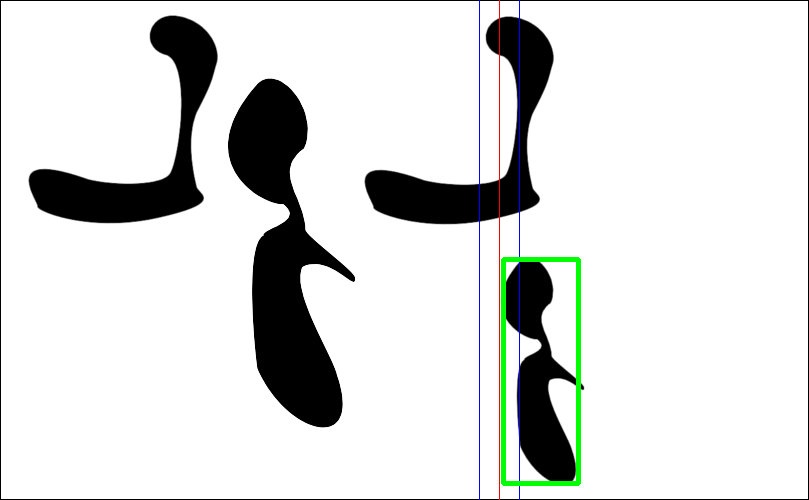
\includegraphics[angle=0,width=0.55\textwidth]{afsnit/afprovning/billeder/naive_losning/naiv_blob1.png}
        	\label{naiv_blob1}}\hspace{1em}
    		\subfloat[Værgen den lille region eller den store er fundet]{
	        	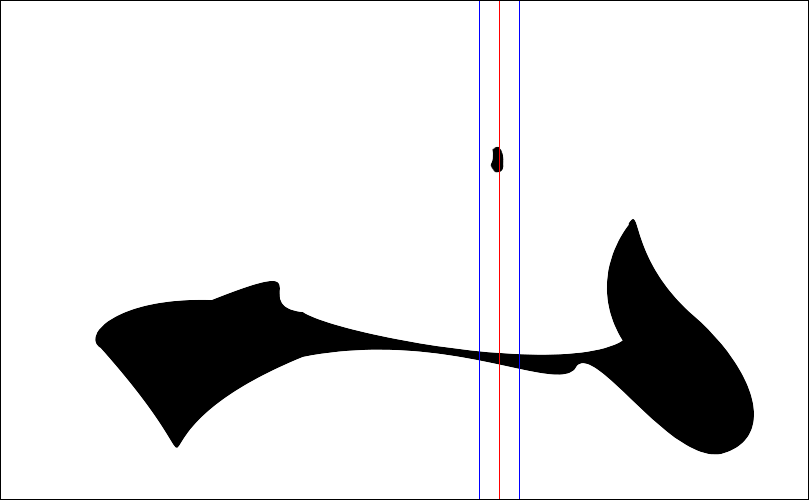
\includegraphics[angle=0,width=0.55\textwidth]{afsnit/afprovning/billeder/naive_losning/naiv_blob2.png}
	       	\label{naiv_blob2}}\hspace{1em}
    		\subfloat[Kun den nederste højrisondt er fundet]{
	        	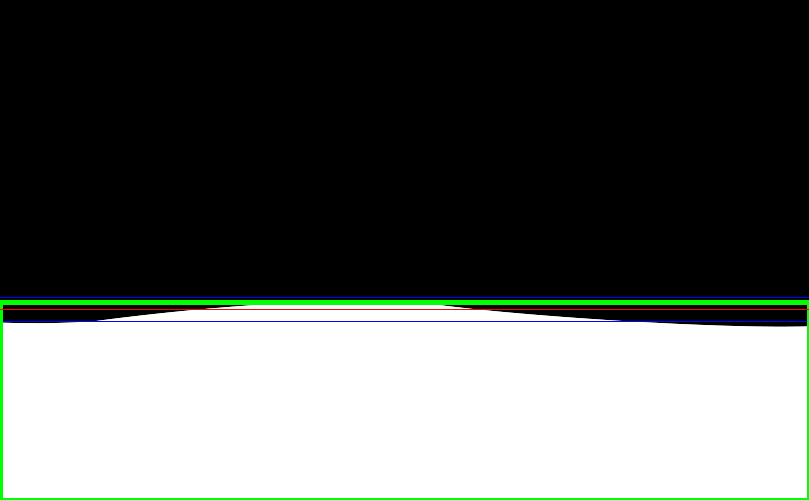
\includegraphics[angle=0,width=0.55\textwidth]{afsnit/afprovning/billeder/naive_losning/naiv_hoisont1.png}
		    \label{naiv_hoisont1}}\hspace{1em}
		    \subfloat[2 regioner hvor den ende er sorteret vær på grund af dens masse]{
	        	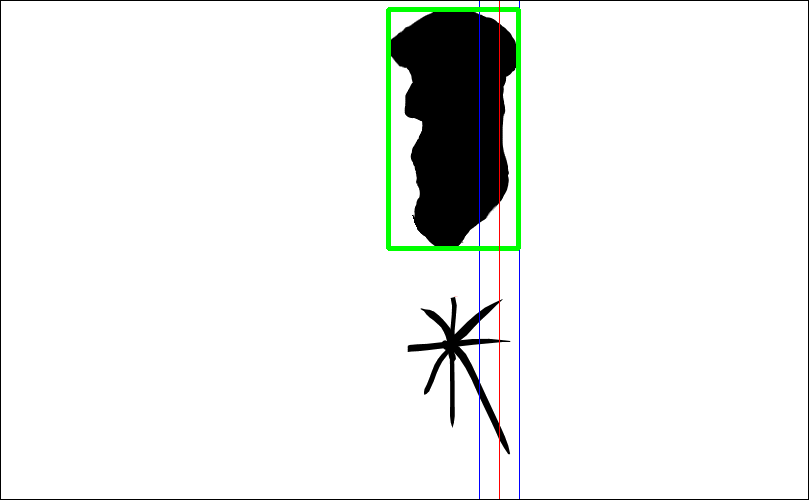
\includegraphics[angle=0,width=0.55\textwidth]{afsnit/afprovning/billeder/naive_losning/naiv_mass.png}
	       	\label{naiv_masse}}\hspace{1em}
        \caption[]{4 test billeder som også blev brugt til at illustrere den naive løsnings fremgangs måde, grån kasse rund om region, betyder at den er taget med af dem naive løsning}
     \label{naiv_detektion_test}
\end{figure}
\clearpage

\subsection{Afprøvning på malerier}
For at se på hvordan den naive metode virker på malerier afprøver vi den
på 6 malerier, først på 3 malerier, hvor regions detektoren virker
efter vores hensigt og så på 3 malerier, hvor region detektoren ikke
virker. Beskrivelsen af hvad der sker i billedet vil stå i caption


\begin{figure}[h!!]
	\begin{center}
		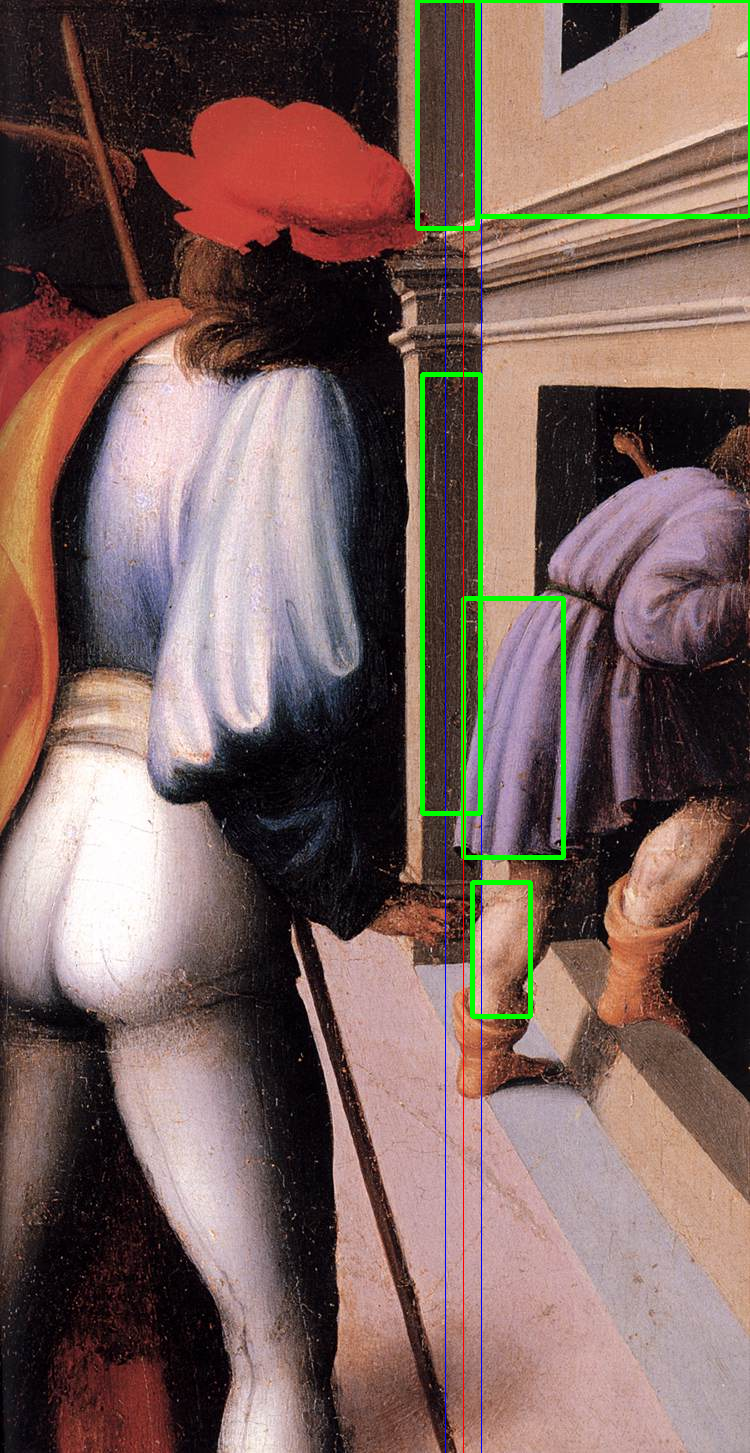
\includegraphics[scale=0.3,angle=0]{afsnit/afprovning/billeder/naive_losning/naiv_kfarver_sdetaljer.png}
	\end{center}
	\caption[]{5 ud af de 6 store regioner fra figur \ref{GRD_virker1} valt til at ligge i snittet, skoene er få små til at blive taget i betragtning}
	\label{naiv_kfarver_sdetaljer}
\end{figure}

\begin{figure}[h!!]
	\begin{center}
		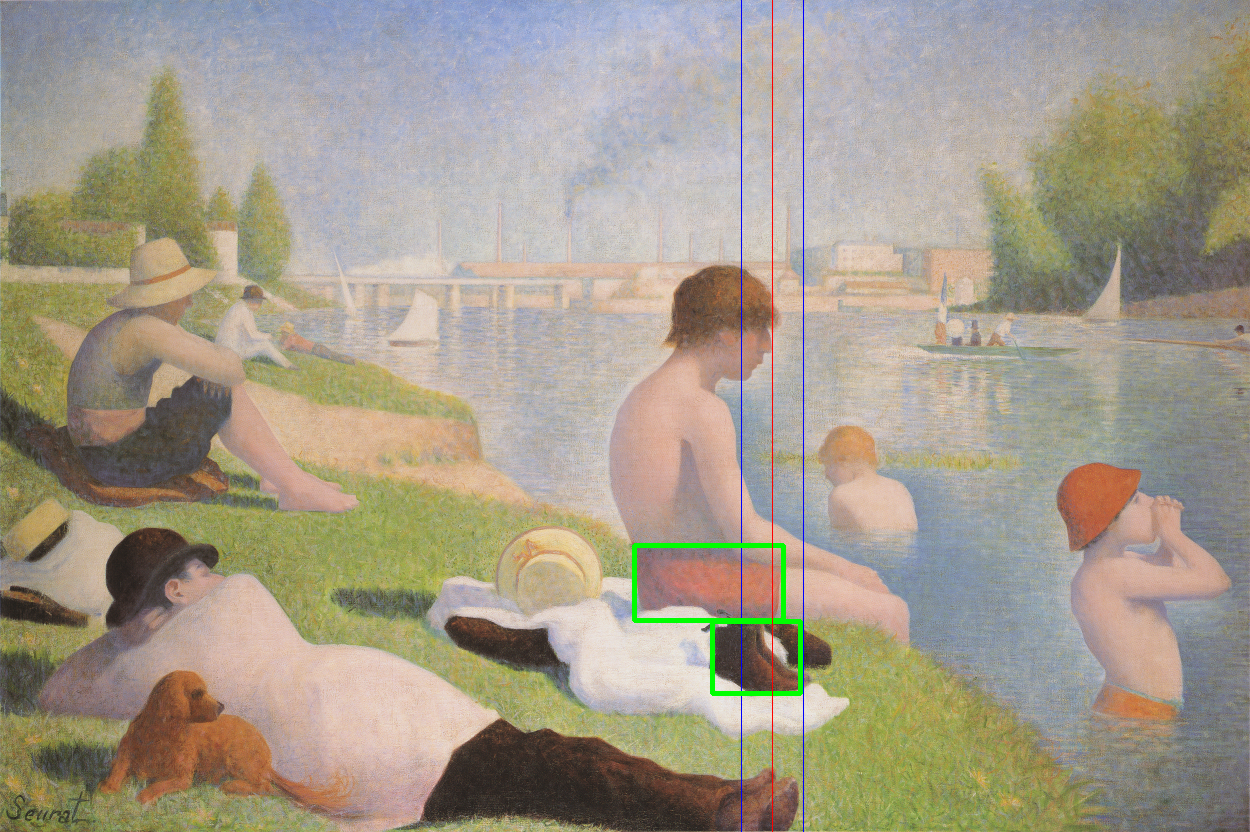
\includegraphics[scale=0.3,angle=0]{afsnit/afprovning/billeder/naive_losning/naiv_mfarver_mdetaljer.png}
	\end{center}
	\caption[]{Bukserne og skoene er tager med af den naive løsning, men drengen er sorteret vær da har krydser snittet}
	\label{naiv_mfarver_mdetaljer}
\end{figure}

\begin{figure}[h!!]
	\begin{center}
		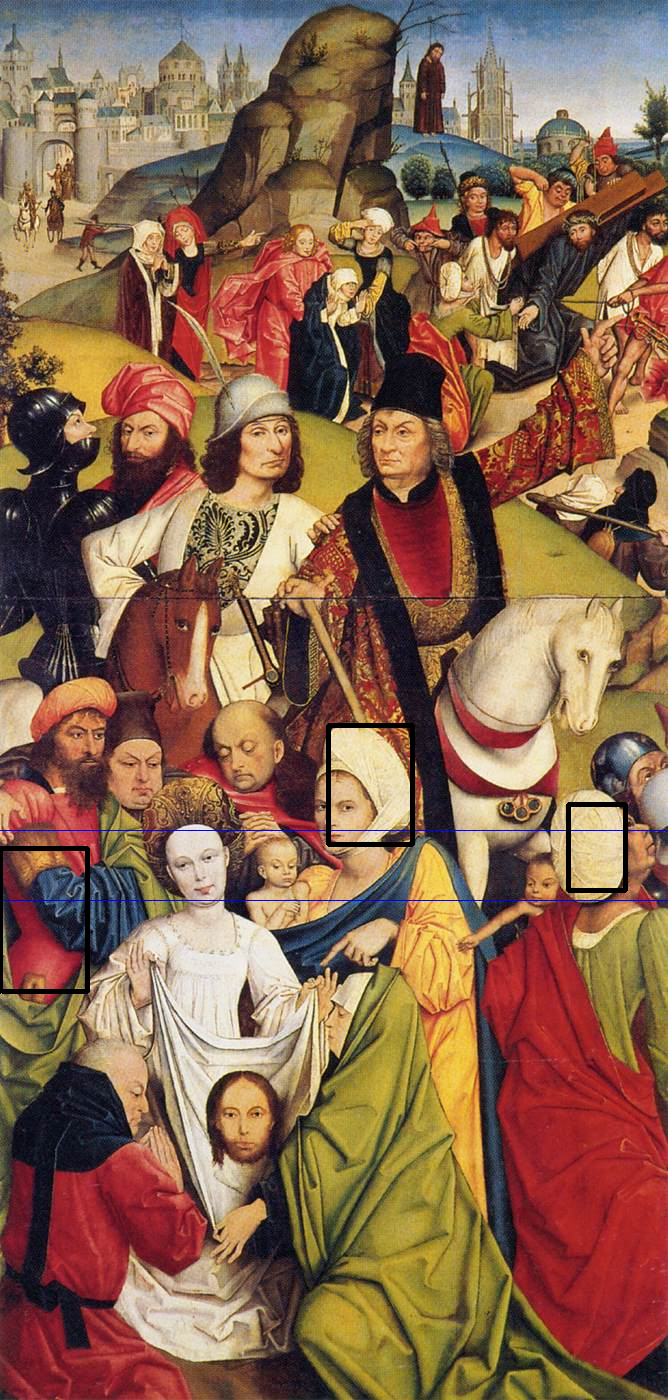
\includegraphics[scale=0.3,angle=0]{afsnit/afprovning/billeder/naive_losning/naiv_kfarver_kdetaljer.png}
	\end{center}
	\caption[]{Et billedet med mange hoder i snittet, hvor 2 af dem bliver godtaget af den naive metode til at ligger i snittet, en trøje bliver desværre også taget med »»(måske noget med at der bliver soteret få mange hover fra)}
	\label{naiv_kfarver_kdetaljer}
\end{figure}

\begin{figure}[h!!]
	\begin{center}
		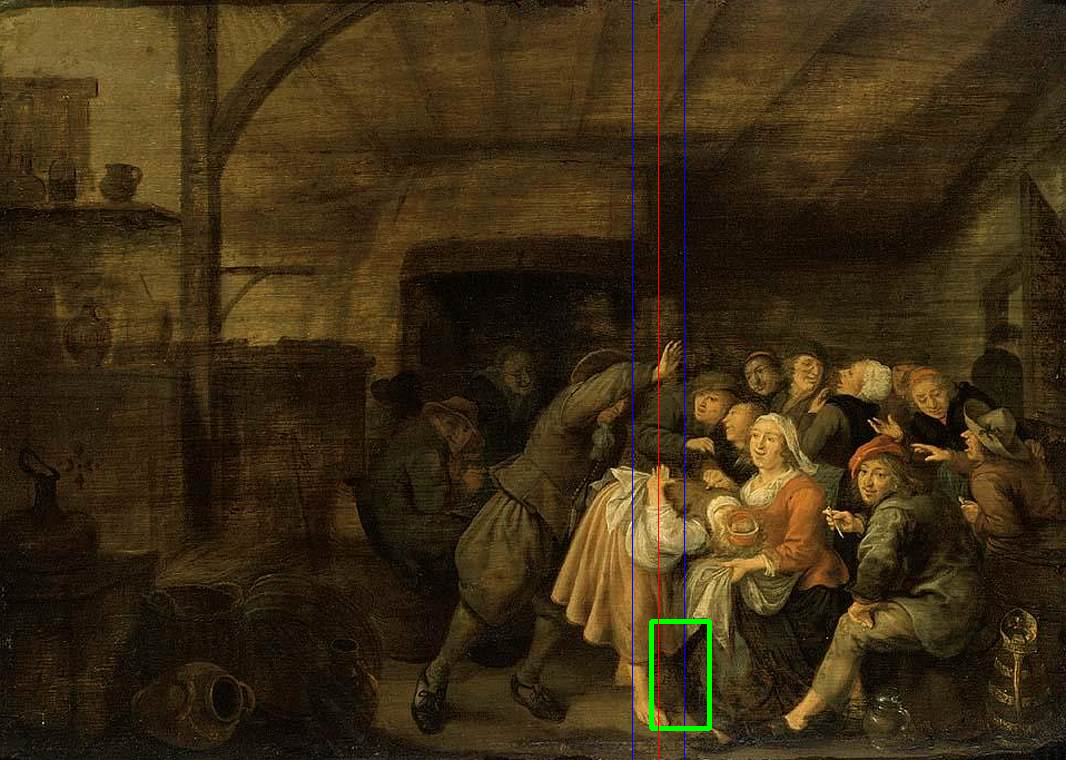
\includegraphics[scale=0.3,angle=0]{afsnit/afprovning/billeder/naive_losning/naiv_virker_ikke1.png}
	\end{center}
	\caption[]{Mallerie hvor region detektor ikke virker, den naive løsning godtager tager en region som ligger helt forkert }
	\label{naiv_virker_ikke1}
\end{figure}

\begin{figure}[h!!]
	\begin{center}
		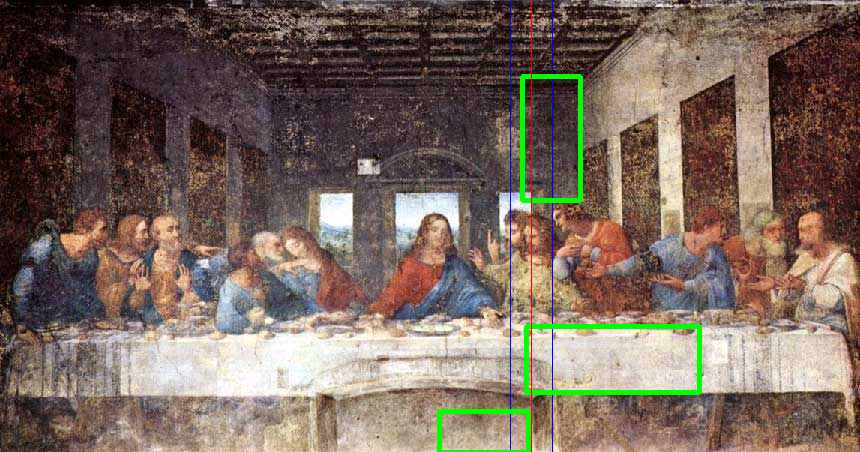
\includegraphics[scale=0.3,angle=0]{afsnit/afprovning/billeder/naive_losning/naiv_virker_ikke2.png}
	\end{center}
	\caption[]{3 regioner bliver godtaget, selv om de ikke er særlige intresante ««(er det ikke en farlige ting at sige )}
	\label{naiv_virker_ikke2}
\end{figure}

\begin{figure}[h!!]
	\begin{center}
		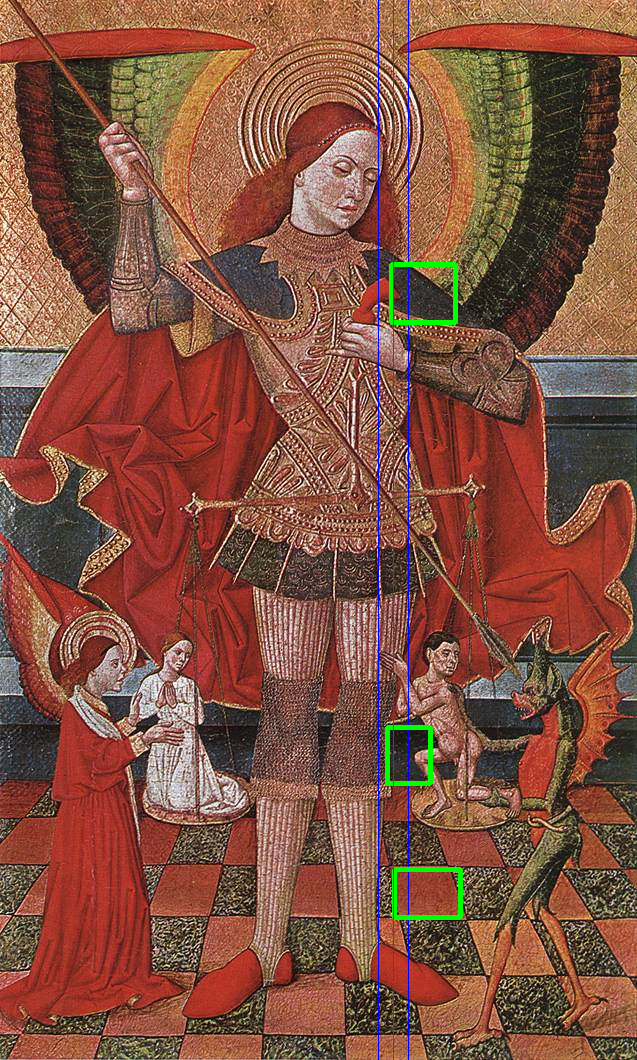
\includegraphics[scale=0.3,angle=0]{afsnit/afprovning/billeder/naive_losning/naiv_virker_ikke3.png}
	\end{center}
	\caption[]{Der bliver fundet 3 region, hvor kun en af dem passer på en ting i billedet}
	\label{naiv_virker_ikke3}
\end{figure}
\clearpage

\subsection{konkulution}
Det virker som om den naive løsning virker efter vores entationer dog
med nogle få falske positive, hvis region detektoren virker på
malerierne, dog fejler den på malerier hvor region detektoren fejler, og
kommer med en masse falske positive.
